\documentclass{article}
\usepackage{amsfonts,amsmath, amssymb, xcolor, amsthm,}
\usepackage{atbegshi,picture}
\addtolength{\topmargin}{-.25in}
\usepackage[margin=1in]{geometry}
\usepackage{mathrsfs}
\usepackage[mathscr]{euscript}
\usepackage{enumerate}
\usepackage{cleveref}
\usepackage{listings}
\usepackage{graphicx}
\lstset{
  basicstyle=\ttfamily,
  mathescape
}
\usepackage{tikz}
\usepackage{ wasysym }
\newcommand*\circled[1]{\tikz[baseline=(char.base)]{\node[shape=circle,draw,inner sep=2pt] (char) {#1};}}
\begin{document}
\newtheorem{lemma}{Lemma}
\newtheorem{sublemma}{Lemma}[lemma]
\begin{flushleft}
AUSM RHD Notes
\end{flushleft}
\begin{center}
\line(1,0){450}
\end{center}

\begin{enumerate}
  \item Naive approach to AUSM in RHD.
        The Method is exactly the same, only difference is Flux, $H$, and $a$ are modified for the RHD case.
        \begin{figure}[h]
    \centering
    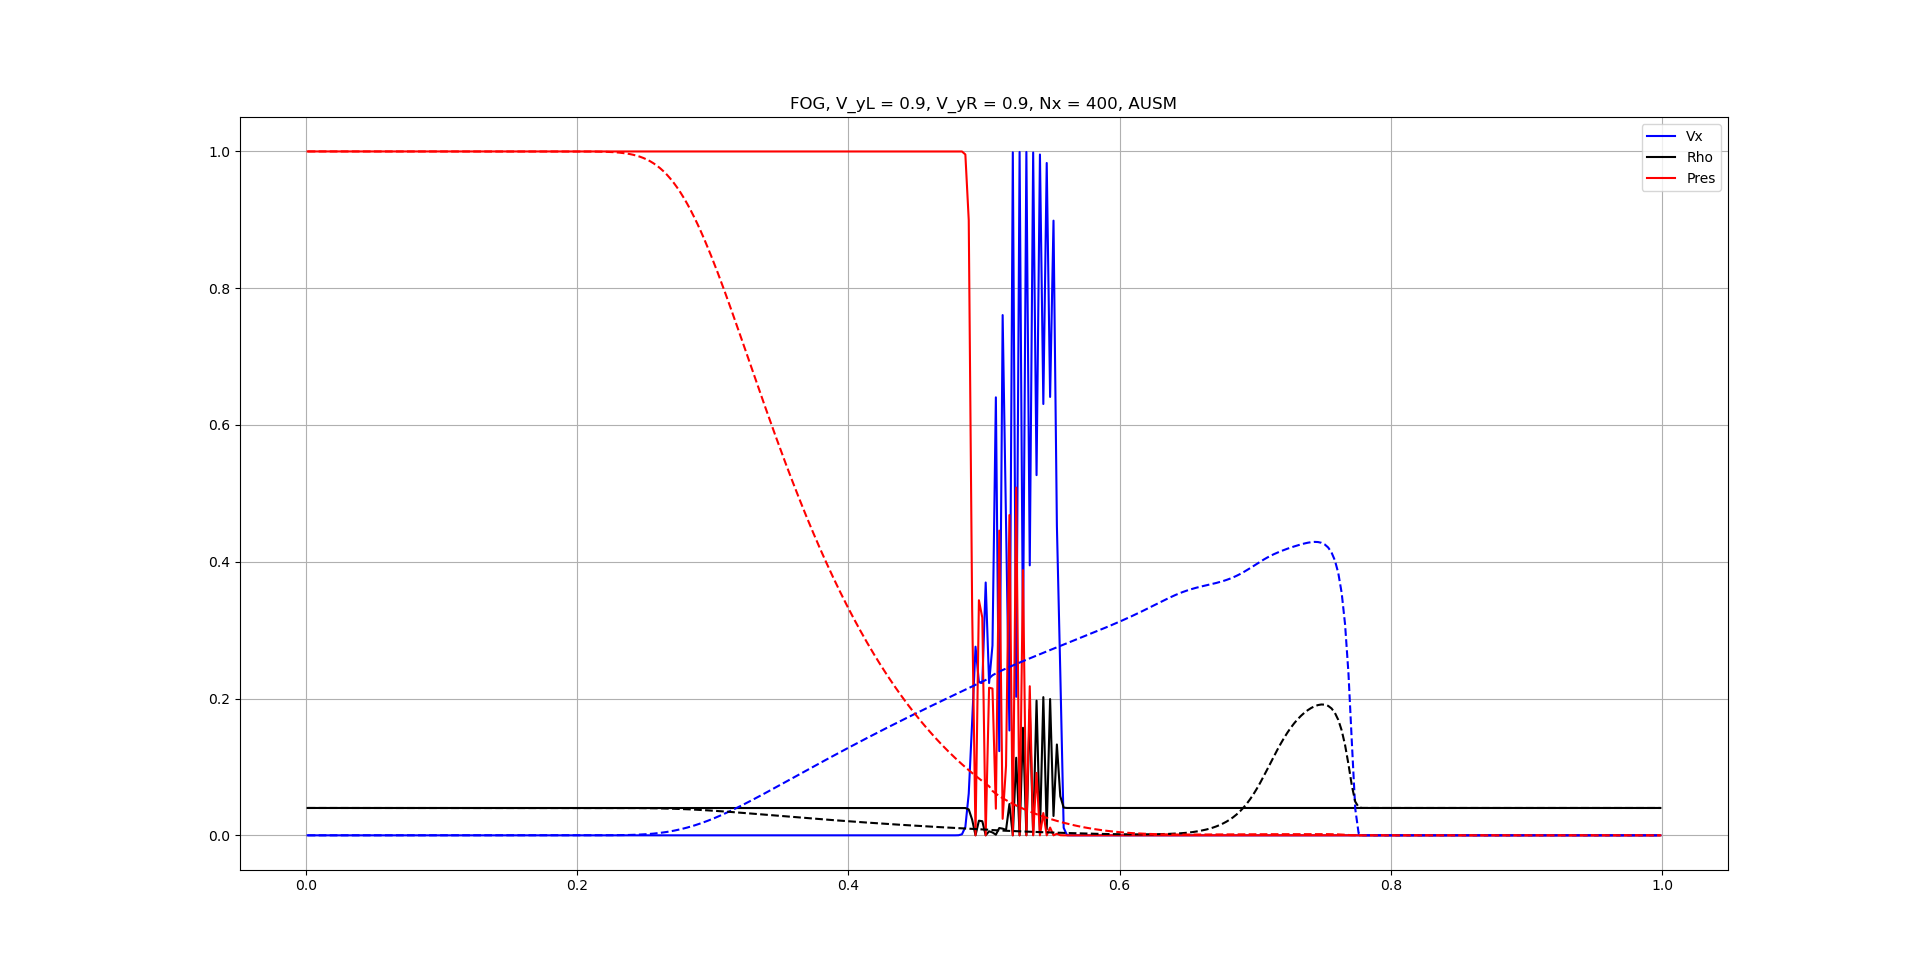
\includegraphics[width=.9\textwidth]{Fig1.png}
    \caption{Dashed Lines are HLLC. So I don't think this is great}
    \label{fig:mesh1}
\end{figure}

\end{enumerate}

Ok, Fixed the problem. I forgot to remove the $u_{x}$ from the flux. Resolving that the result looks better.
\begin{figure}[h]
    \centering
    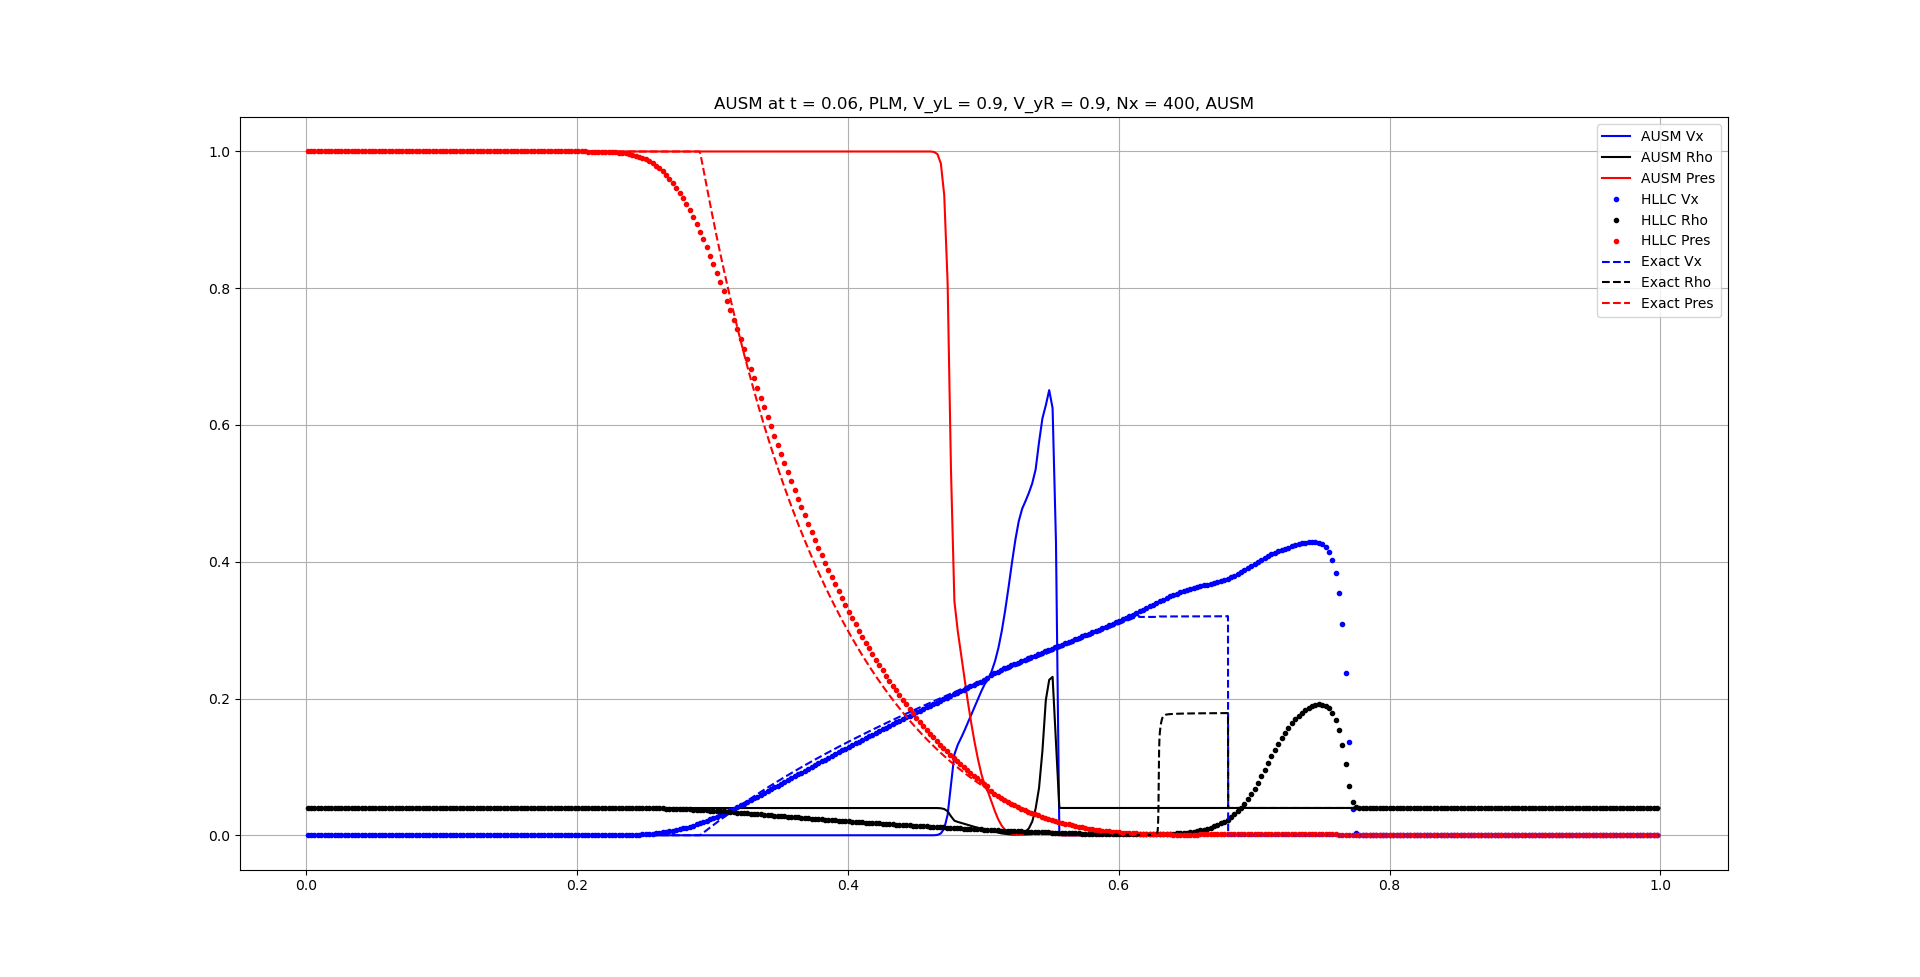
\includegraphics[width=.9\textwidth]{Fig2.png}
    \caption{Good Start For AUSM at T = 0.06}
    \label{fig:mesh1}
  \end{figure}

  Around T = .14 We get oscellations in AUSM which cause eventual failure.

  \begin{figure}[h]
    \centering
    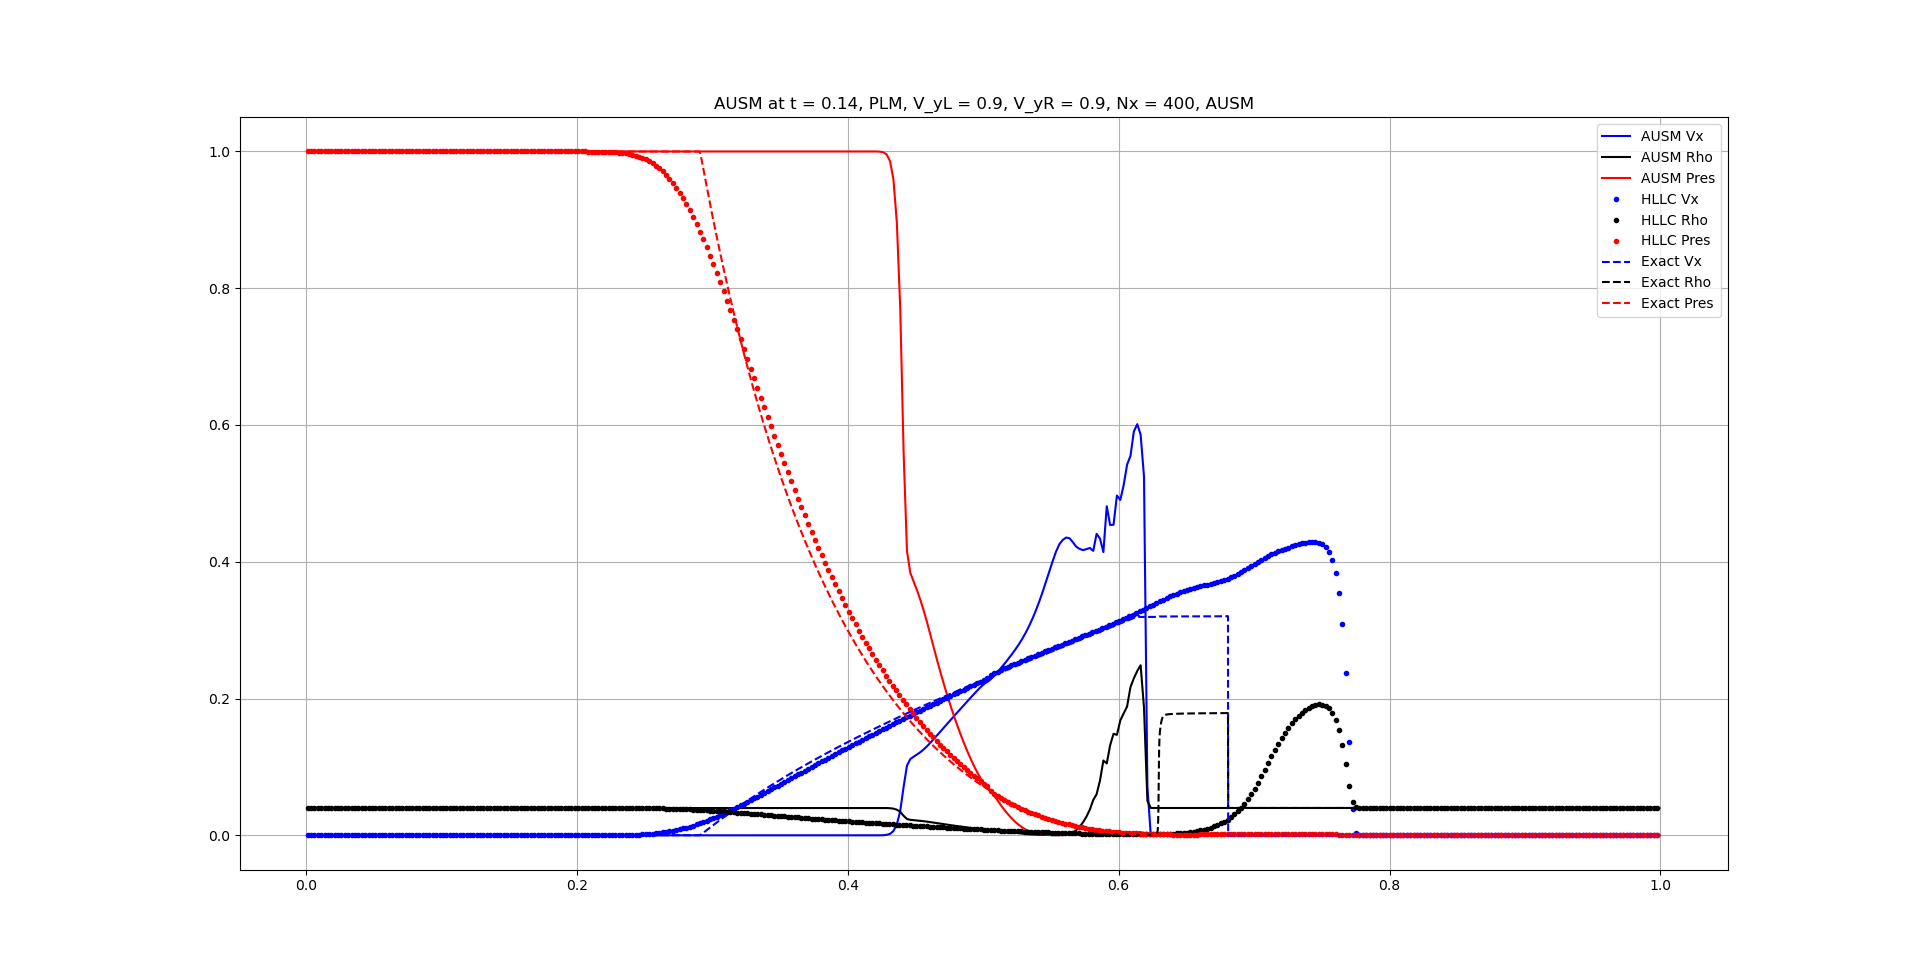
\includegraphics[width=.9\textwidth]{Fig3.png}
    \caption{Wiggles show up at T = 0.14}
    \label{fig:mesh1}
  \end{figure}

  \begin{figure}[h]
    \centering
    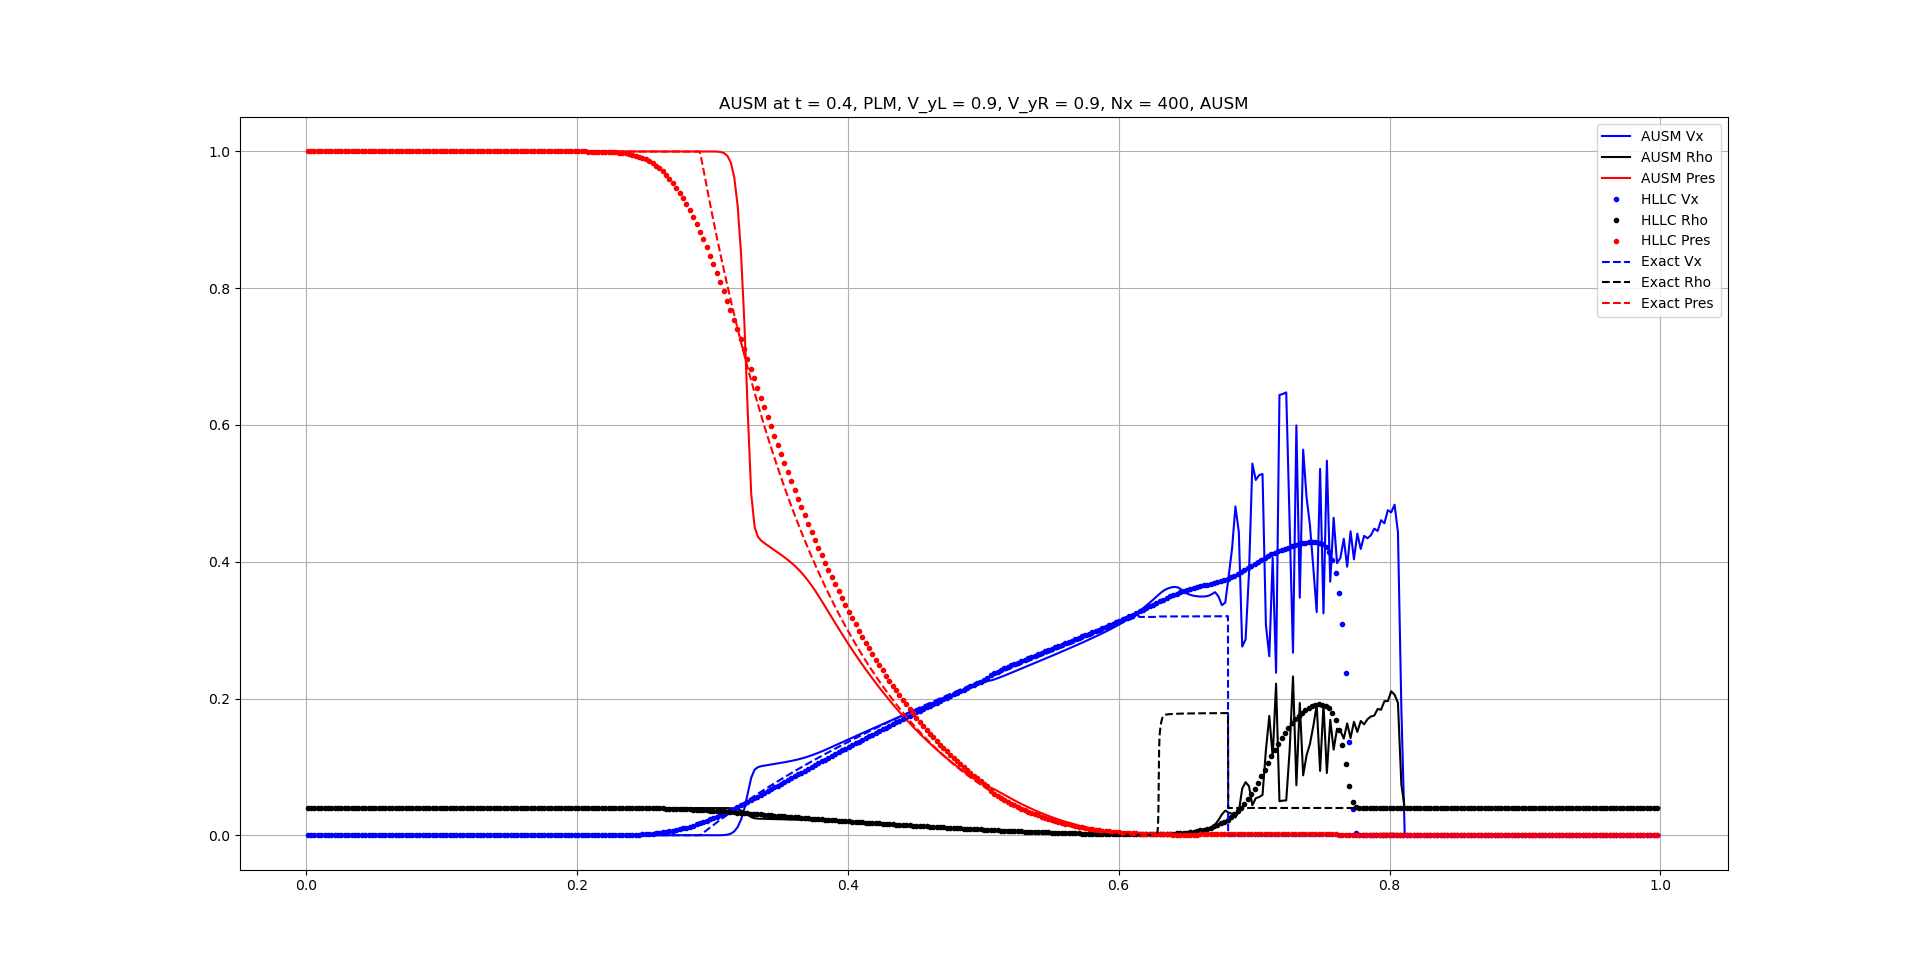
\includegraphics[width=.9\textwidth]{Fig4.png}
    \caption{Ausm bad at T = 0.4}
    \label{fig:mesh1}
  \end{figure}

  Solution is much better using FOG

  \begin{figure}[h]
    \centering
    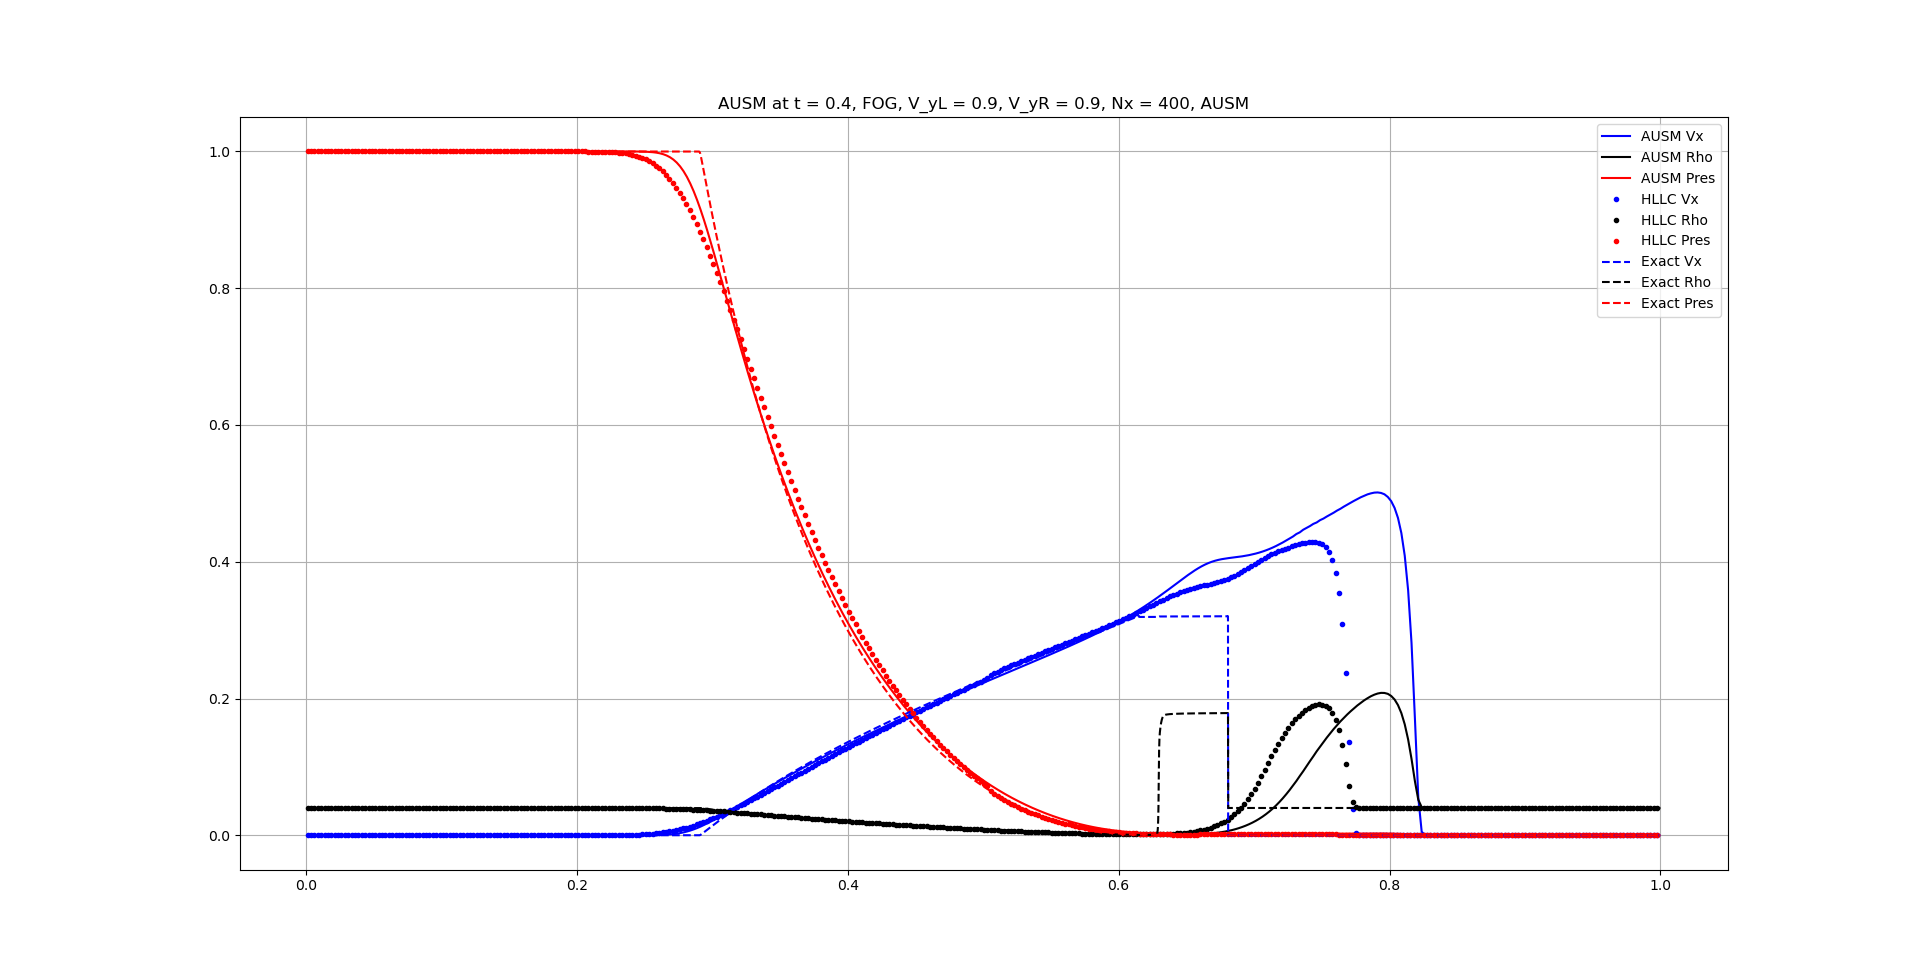
\includegraphics[width=.9\textwidth]{Fig5.png}
    \caption{Disturbingly we see the shock moving even faster than with HLLC}
    \label{fig:mesh1}
  \end{figure}
\end{document}
